\chapter{Neutronic Optimization}
\label{ch:GAOpt}
\section{Introduction}
A single film does not have the necessary interactions to fulfill the neutron count rate criteria multiple films are necessary, and the arrangement of these films provides a design space for a replacement RPM.
In the case of the RPM, there are several design parameters that can be explored:
\begin{itemize}
  \item the neutron absorber loading of the film,
  \item the thickness of the film,
  \item the geometry of the film (cylinders or sheets), and
  \item the placement of the films.
\end{itemize}
It is expected that the loading of the film will be limited by the optical clarity, and that the thickness of the film will be determined by the optimization of the energy deposition.
Thus, of the above design parameters only the geometric placement of the films is an available optimization space.

%% How do I want to do the differnet geometries?
They are generally a vertical or horizontal layer of the films or a vertical or horizontal arrangement of the films arranged in concentric cylinders.
Several possible geometries have been considered for the films. 

Preliminary work by this author provided a simple design in which the detector layers are linearly placed throughout the detector volume in an alternating fashion.
The analysis of the neutron flux throughout this detector lead to a flat flux profile as shown in \autoref{fig:AltLayerThermalNeutronFraction}.
\begin{figure}
  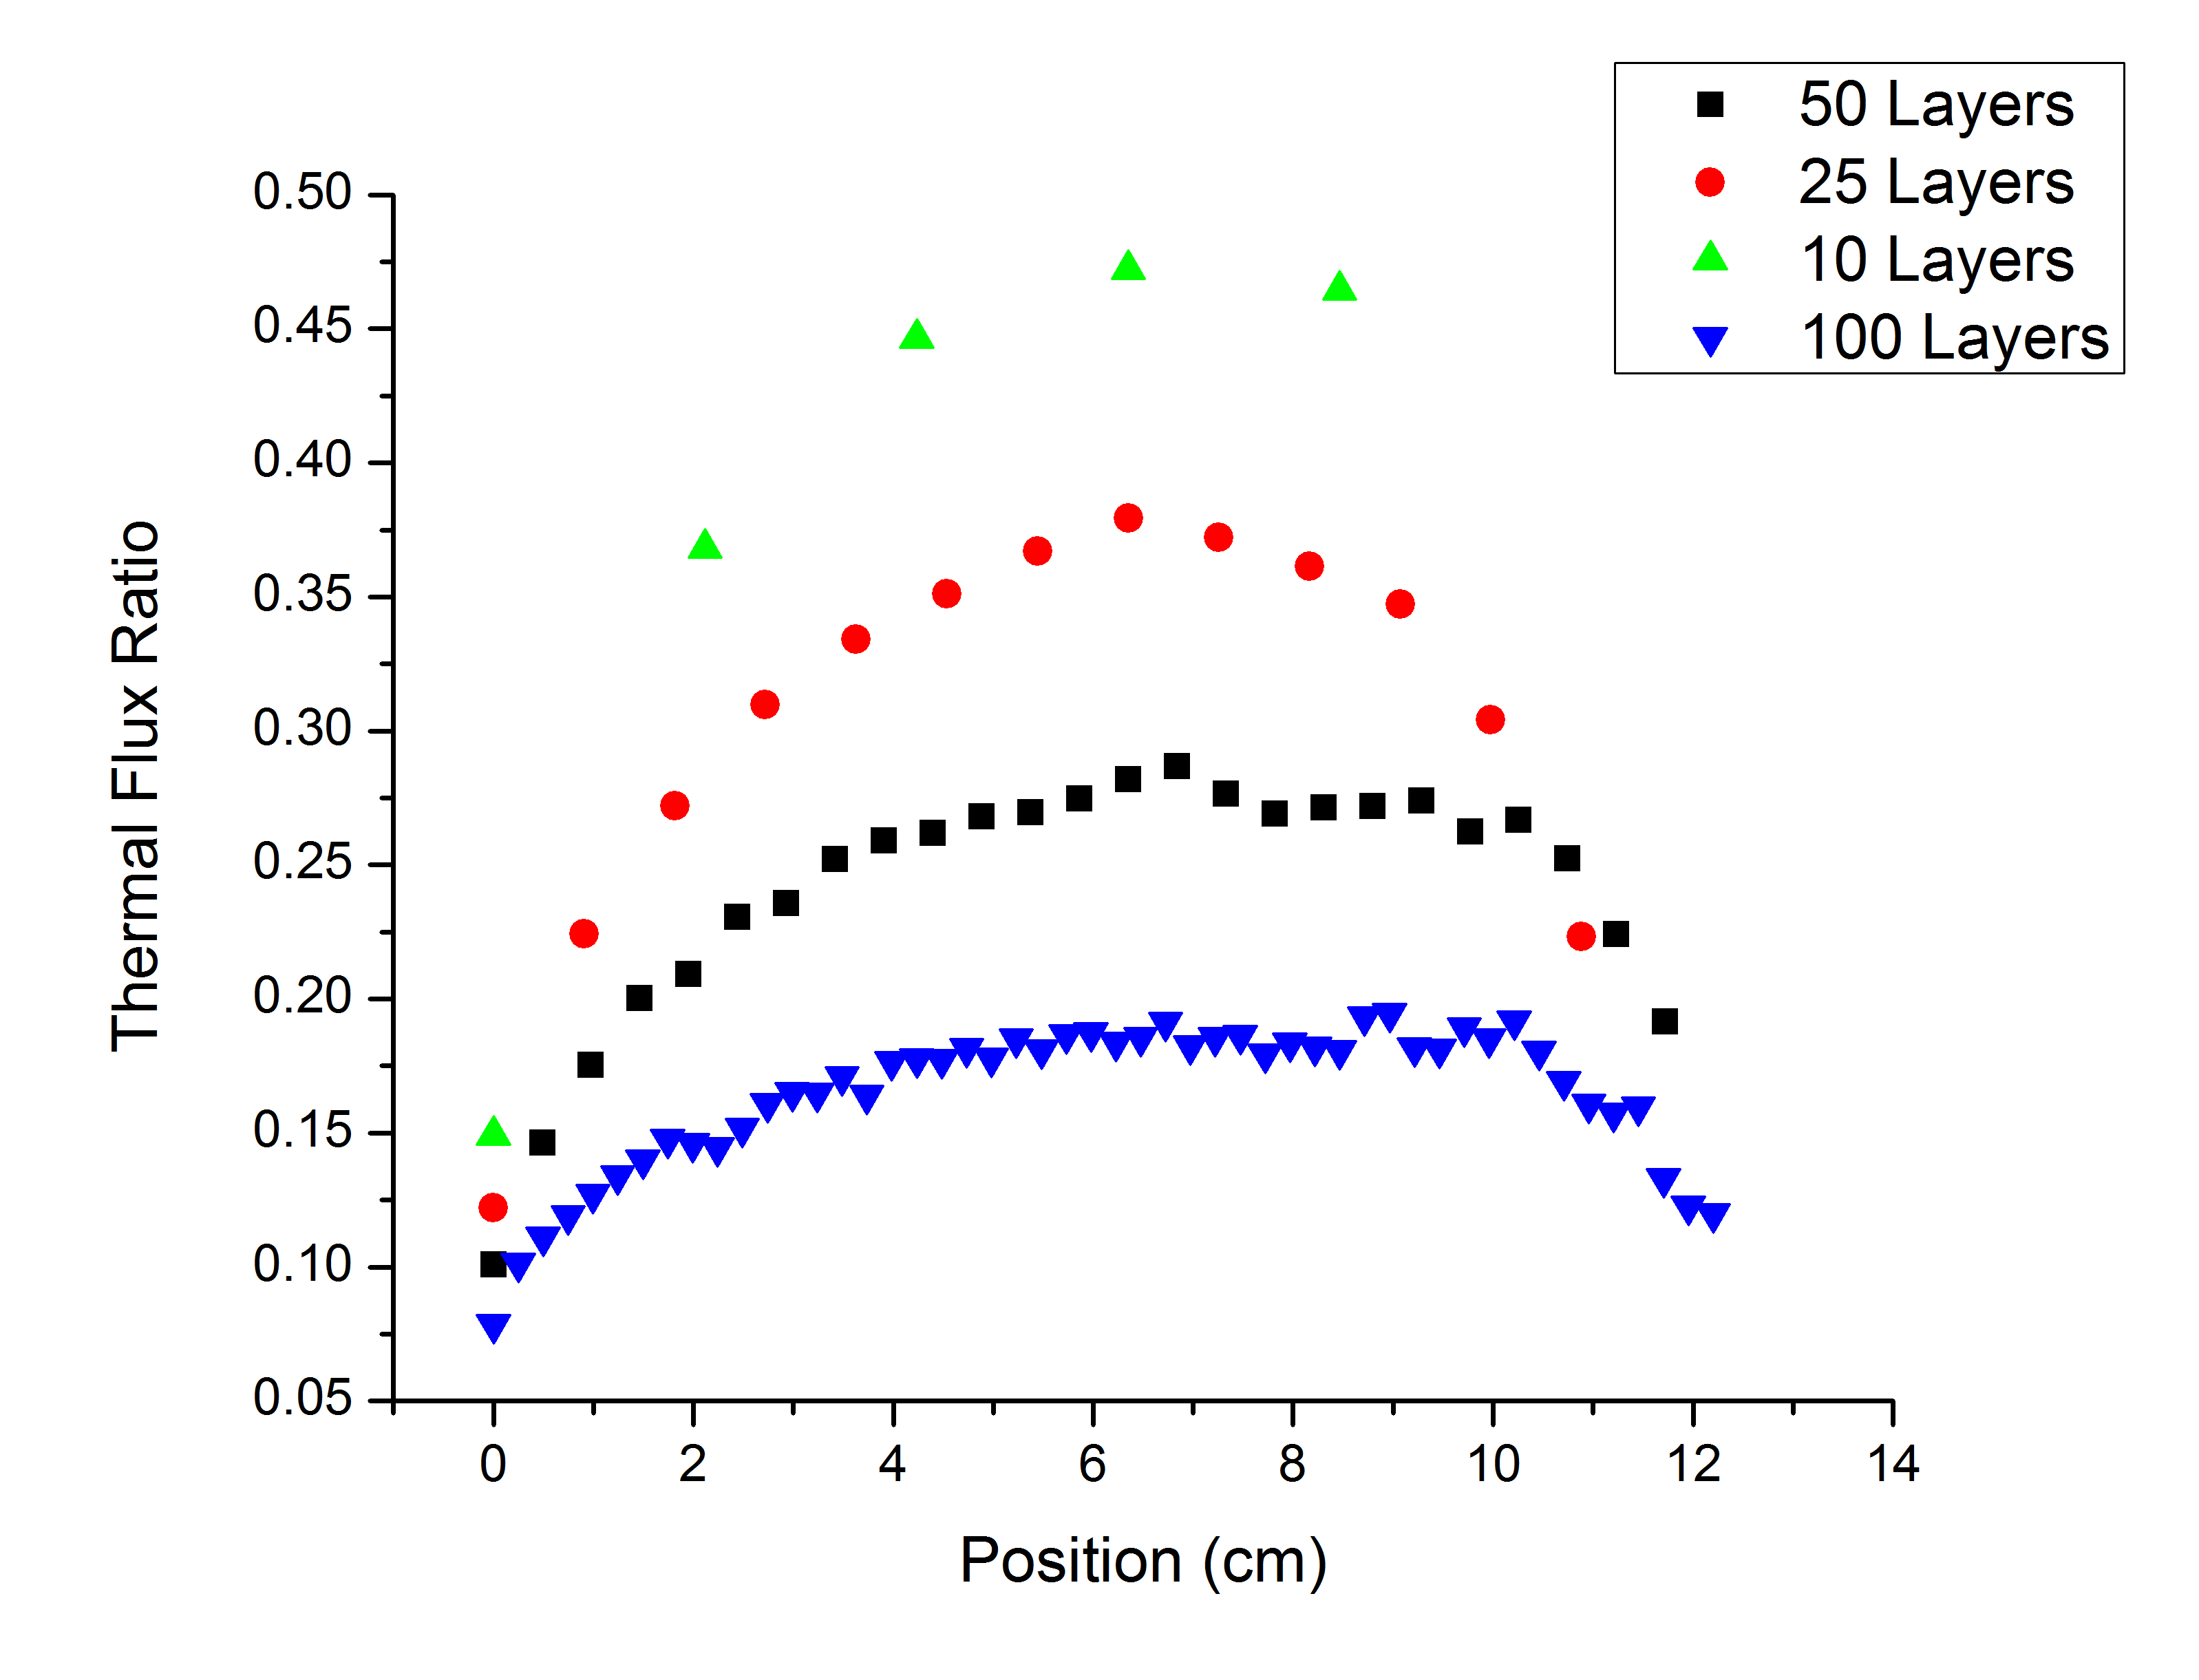
\includegraphics[width=\textwidth]{ThermalFluxRatioAltLayers}
	\caption{Fraction of the neutron flux that is thermalized through a alternating detector and moderator layered RPM.  The low thermal fluxes result in a poor utilization of the high thermal cross section of \iso[6]{Li}.}
	\label{fig:AltLayerThermalNeutronFraction}
\end{figure}
Effective utilization of the neutron flux is necessary for minimizing the amount of neutron absorber (\iso[6]{Li}) that is used in the detector.
Several different strategies can then be used to optimize the geometry to ensure effective utilization of the thermal cross section of the absorber material.

In this particular problem the placement of a film greatly changes the solution because of the large change in the neutron flux, and traditional gradient based solvers would tend to be trapped in these local minima.
Genetic algorthims were chosen as the optimization technique because they are less suscutible to local minimas than other search techniques and tend to preform very well on combinitorial problems such as this one \cite{Mitchell}.

\section{Genetic Algorithm Introduction}
Genetic algorthims provide a search technique analagous to biological evolution in which instead of searching from general to specific solutions, or from more simple to complex, genetic algorthims generate solutions by mutating and combining parts of the best previously known solutions.
At each step in the search for the best solution a collection of solutions called the current \textit{population} is refined by replacing members with solutions representing the offspring of the best individuals.
The goals is then to find the best solution to the problem as determined by some criteria, called the \textit{fitness function}.
The genetic algorithm typically consist of four tasks: creating an initial population, evaluating that populations fitness, selecting members of the current population to breed, and then applying genetic operators to the selected members to breed the new population. 
This is completed until either a maximum generation is reached or the desired fitness is achieved, as shown in \autoref{alg:GAOutline}.
\begin{algorithm}
  \caption{Genetic Program Outline}
  \label{alg:GAOutline}
  \begin{algorithmic}
    \WHILE{$error>goal$}
      \FORALL{$t\in F$}
        \STATE{Compute fitness}
      \ENDFOR
      \FORALL{$t\in F$
        \STATE{Choose individuals based on fitness}
      \ENDFOR
      \STATE{Select individuals for next population}
      \STATE{Crossover selected individuals}
      \STATE{Mutate selected individual}}}
    \ENDWHILE
  \end{algorithmic}
\end{algorithm}

\subsection{Problem Representaiton}
The thickness of the RPM  (\SI{12.7}{\cm}) was divided into slices, where each slice could be either a detector slice or a moderator slice.
These slices of detector material (represented as a \verb+1+) or moderator material (represented as a \verb+0+) were appened into a sequence.
This sequence of one's and zero's (or bit string) then completely represented the goemetry of the RPM and formed the basis for all possible solutions to the optimization problem.
For example the sequence \verb+0001110010+ would represent a detector that had three moderator slices, three detector slices, another two moderator slicees, and a final detector slice before a single moderator slice as the reflector.
Examples of two differnet genomes are shown in \autofref{fig:ExGeoGenomes}
\begin{figure}

  \caption[Example Geometries Genomes]{Example of Geometry Genomes}
  \caption{fig:ExGeoGenomes}
\end{figure}
In terms of genetic algorthims the set of all possible solutions is refered to as the \textit{genome}.
The length of the genome is thus the number of slices in the geometry, where a higher length genome allows for a more complicated geoemtry.
The intial population for the genetic algorthim was initialized to be random bit strings with equal probability of a slice being a detector slice or moderator.

\subsection{Population Selection}
Several differnet selection technqiues are available to select the individuals from one population to reproduce in the next.
Among the most common are fitness proportional selection (roulette selection) and tournament selection.
Roulette selection occurs when the individuals are ranked by their fitness, and individuals are chosen by their fitness rank.
This is analagous to a roulette wheel where the space a canidate occupies on the wheel is proporitional to its fitness.
Higher fitness individuals will occupy more space, and will thus have a higher probability of being selected.
Tournament selection is another selection techinque in which a pool of solutions are chosen at random from the current population.
Within this tournament pool a fitness proportional selection will be used to select individuals for the next generation.
The fitness function will be explained in detail in \autoref{sec:FitnessFunc}.

\subsection{Genetic Operators}
Individuals selected for reproduction are subjected to genetic operators to breed the next generation. 
Genetic programs generally contain two genetic operators, crossover and mutation. 
Crossover serves to create new members of the population by interchanging the genetic material of two parents in which significant changes in the solutions are achieved. 
Mutation serves to slightly modify an existing solution. 

Crossover is defined in genetic programming as the swapping of genetic material from one individual to another.  
For bit strings several crossover operations are commonly used; they are 1) single point crossover, 2) two point crossover, and 3) uniform crossover.
An example of the crossover operations are shown in \autoref{fig:GeneticCrossover}.
In single point crossover a single point is selected on both parents genes and the genetic material between the two parents is swapped.
In two point crossover two points are chosen on the parents bit strings and the genetic material is swapped between the intervals.
Uniform crossover uses a set mixing ratio for which according to that ratio an individual bit will be interchanged between the two parents to yeild the dauthers.
\begin{figure}
  \begin{subfigure}[b]{0.3\textwidth}
    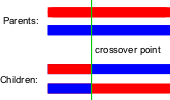
\includegraphics[width=\textwidth]{SinglePointCrossover}
    \caption{Single Point Crossover}
  \end{subfigure}
  ~
  \begin{subfigure}[b]{0.3\textwidth}
    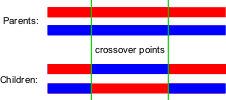
\includegraphics[width=\textwidth]{TwoPointCrossover}
    \caption{Two Point Crossover}
  \end{subfigure}
  ~
  \begin{subfigure}[b]{0.3\textwidth}
    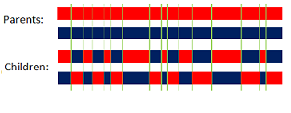
\includegraphics[width=\textwidth]{UniformCrossover}
    \caption{Uniform Crossover}
  \end{subfigure}
  \caption[Genetic Crossover Operations]{Genetic Crossover Operations. Images from Wikipedia}
  \label{fig:GeneticCrossover}
\end{figure}

Mutation is used to produce small, random changes in the genomes to maintain genetic diversity.
The mutation operation was chosen to be a simple bit flip in which a randomly chosen \verb+1+ or \verb+0+ in the geoemtry was flipped; for example \verb+001001010+ could be mutated to \verb+001001000+.
Generally the mutation rate is set very low (less than 2\%) in order to prevent the search for the solution to becoming simply a random search.
In this representation of the problem a mutation produces a very large change in the solution and the mutation rate was set even lower.

\subsection{Fitness Function}
\label{sec:FitnessFunc}
The fiteness function defines the criteria for ranking solutions and probablistically including them in the next generation.
The fitness function was choosen to count rate per mass of \iso[6]{Li}, provided that the geometry meet the total count rate criteria.
If it failed to meet the count rate criteria a zero fitness was returned \eqref{eqn:FitnessFun}.
\begin{align}
    \label{eqn:FitnessFun}
    f(\vec{x})
    = \begin{cases}
    0 & \text{if} \text{countRate}(\vec{x}) \leq \SI{2.5}{cps\per\nano\gram\iso[252]{Cf}} \\
    \text{countRatePerMass}(\vec{x})
    \end{cases}
\end{align}
Films that have excessive detector laysers will be penalzied by the normalization by the mass of \iso[6]{Li} that they contain, while favoring films that have the minimium number of detector layers that meet the count rate criteria and have a more effective utilization of the neturon flux which increase their count rate.

At this point it is instructive to make a note about the size of the solution space.
\autoref{tab:BitStringGeo} some of the these geometries are simple enougth that the search space can be computed exaustively.
\begin{table}
    \caption[Genome Bit String Geometries]{Bit String Simplified Geometetry Descriptions}
    \label{tab:BitStringGeo}
    \centering
    \begin{tabular}{ c | c cc}
     \toprule
     Genome Length&Slice Thickness&Possible Geomeries \\
     \midrule
        5&2.54&31\\
        10&1.2700&1,023\\
        15&0.8467&32,765\\
        20&0.6350&1,048,575\\
        25&0.5080&33,554,431\\
        30&0.4233&\num{1.07E9}\\
        35&0.3629&\num{3.44E10}\\
        40&0.3175&\num{1.10E12}
    \bottomrule
    \end{tabular}
\end{table}
There are several salient features highlighted in \autoref{tab:BitStringGeo}.
For small genome lengths (less than 10) it is possible to exhasutive search the hypothesis space of possible solutions.
This is not possible for the larger genome lengths.
Thefore, efficient evaluation of the fitness function is necessary in order to evolve a reasonable number of solutions.
In addition the refinement in the details of the geometries increases lineary with the genome length while the size of the search space increases as $2^n$.
This suggest that a hybrid method of finding a basic geometry in a low search space and then preforming pertubations on that geometry will have a better performance than attempting to search the higher geometry solutioin space.

\section{Neutronic Models}
The interaction rate of a geometry can be found by solving the neutron transport equation in that geometery and then composing the neutron flux with the absorber materials reaction rate.
Thankfully, models have already been developed for this purpose.
Deterministic models discretize the transport equation into energy groups and quadrature sets or spherical harmonics, and then solve the discritized equations.
Probabilistic models follow the path of indvidiuals neutrons with interactions based on the probability of a given event occuring.
Such codes are also known as Monte Carlo models, for which MCNPX is a well known example.
A full 3D Monte Carlo treatment of the problem provides an accurate knowledge of the interaction rate at the expense of higher computation times. 
In order to preform a faster search of the parameter space a simple one dimenensional model was desired.
XSDRN, a one dimension discrete ordiantes that solves the one dimensional Boltzmann equation distributed in the SCALE package was chosen for this purpose.
XSDRN will be used to preform an initial parameter study and determine a subset of optimal geometries on which to preform more accurate Monte Carlo (MCNPX) modeling. 
A subset of the highest preforming geometries validated by the detailed model with then be used to test the sensitivity by adjusting the position of the films by fractional amounts.
%%%%%%%%%%%%%%%%%%%%%%%%%%%%%%%%%%%%%%%%%%%%%%%%%%%%%%%%%%%%%%%%%%%%%%%%%%%
%                                                                         %
%                             XSDRN Model                                 %
%                                                                         %
%%%%%%%%%%%%%%%%%%%%%%%%%%%%%%%%%%%%%%%%%%%%%%%%%%%%%%%%%%%%%%%%%%%%%%%%%%%
% XSDRN Model of the RPM
\subsection{XSDRN Detector Model}
The XSDRN model was a simplified model of the RPM along an axis through the midpoint of the RPM.
A $S_n$ of 16 was used for the quadrature, and convergence for the flux was set at \SI{1E-7} for the inner iterations.
Only two types of materials were simulated in the XSDRN calcualation; a detector material containing the \iso[6]{LiF} and a moderating material of polystyrene.
The 44 group neutron cross sections of each of these materials were processed using NITWAL (without any resonance regions) assuming an infinate, homogenous medium for simplicity.
The XSDRN model consisted of a multi-group isotropic boundary source on the left most boundary on the RPM, with the values for this flux coming from an MCNPX simulaiton.
A MCNPX calculation was used to determine the neutron flux incident upon the left most side of the RPM, and then this flux was input as the surface boundary flux condition in XSDRN.

%The XSDRN model was validated by comparing to the MCNPX simulations of a similar geometry.
%It was observed that geometries that started with a neutron absorber layer did not have good agreement with the MCNPX model; this is attributed to the breakdown of the diffusion equation in a strongly absorbing medium near a source.
%Some strification of the results were also observed, leading to the conclusion that the XSDRN calculations should only be used as a general guide.

%%%%%%%%%%%%%%%%%%%%%%%%%%%%%%%%%%%%%%%%%%%%%%%%%%%%%%%%%%%%%%%%%%%%%%%%%%%
%                                                                         %
%                             MCNPX Model                                 %
%                                                                         %
%%%%%%%%%%%%%%%%%%%%%%%%%%%%%%%%%%%%%%%%%%%%%%%%%%%%%%%%%%%%%%%%%%%%%%%%%%%
% MCNPX Model of the interaction rate
The performance of films is simulated in MCNPX, a Monte Carlo transport code\cite{pelowitz_mcnpx_????}.
The geometry is as in the PNNL reports, namely a nano-gram of \iso[252]{Cf}  encased in \SI{0.5}{\cm} of lead and \SI{2.5}{\cm} of HDPE. 
The size of the RPM8 is \SI{12.7}{\cm} deep, by \SI{30}{\cm} wide and \SI{2}{\m} tall.
The interaction rate, $I_{\text{sim}}$ provides the total number of simulated neutron interactions in the detector and is calculated using the a cell flux tally in MCNPX and a tally multiplier card.
The reaction rate $\iso[6]{Li}\left(\text{n},\text{t}\right)\alpha$ can be calculated by then applying the appropriate input for the FMn card and using an F4 card to calculate $\phi(E)$.
This is in accordance with the direct evaluation of the PNNL criteria, which require a absolute neutron count rate of \SI{2.5}{count\per\second\per\nano\gram\iso[252]{Cf}}.
Note that in this calculation the source strength is set to be \SI{1}{\nano\gram} \iso[252]{Cf}, which has a neutron emission rate of \SI{2.3E3}{neutron\per\second}.
\begin{align}
  \label{eqn:RPM8InteractionRate}
  I_{\text{sim}} &= S_0 I \\
  &= \SI{2.3E3}{neutron\per\second} I
\end{align}



However, not all of these interactions will lead to counts above the pulse height discriminator setting necessary for meeting the gamma intrinsic efficiency.
This is corrected for by scaling $I_{\text{sim}}$ by the fraction of counts, $\eta$, that occur above the gamma LLD \eqref{eqn:FractionOfCountsDefination}, \eqref{eqn:RPMCountRate}.
\begin{align}
  \label{eqn:FractionOfCountsDefination}
  \eta \equiv \frac{\int_{MLLD}^\infty p(x)dx}{\int_0^\infty p(x)dx}
\end{align}
\nomenclature{$p(x)$}{Measured spectra, as a function of channel number}
\begin{align}
 \label{eqn:RPMCountRate}
 \text{Count Rate} &= I_{\text{sim}} \eta
\end{align}

\section{Conclusions}

A physical basis of the optimal solution found by the genetic algorthim can be found by observing the form of the optimal solutions.
These solutions involve an intial moderator layer in order to ensure that all of the neutrons are thermalized to (increasing the thermal fraction by \textbf{SOME PRECENT}).
After this moderator layer a film layer is placed to utilize this neutron spectra; however not all of the thermal neutrons are captured (as the mean free path of a neutron in polyethylene is about \si{0.37}{\cm} and thus some pass through the material) and another abosrber layer is needed to capture those neutrons.  
The neutron flux is then moderated again, and additional layers of detectors are needed to capture this neutron cross section.
However, it is desirably to have a large neutron reflector in the portal monitor to reflect neturons back into the detector slices. 
Theortically this reflector should be as large as possible, but the limited space of the RPM provides a constraint.
A parameter study with a single detector slice between a moderator and reflector constrained by the radiaiton portal monitor design showed that it is desriable to have around \textbf{So much} moderator leaving the majority of the RPM to be left for the reflector.
Thus it is demonstrated that a large reflector is desired.
